\documentclass[12pt]{article}

\usepackage{sbc-template}

\usepackage{graphicx,url}


\usepackage[brazil]{babel}
\usepackage[utf8x]{inputenc}
\usepackage{url}  % para usar URLs nas referencias


\sloppy

\title{Gerenciamento de Processos de Negócio em Cursos de Sistemas de Informação: um Caso Prático\\ Utilizando Software Livre}
%Outra alternativa:
%Utilizando BPM no Processo de Validação de Atividades Complementares em um Bacharelado em Sistemas de Informação

\author{Jessica Lasch de Moura\inst{1}, Gabriel Machado Lunardi\inst{1},\\
Andrea Schwertner Charão\inst{1}, Patrícia Pitthan Barcelos\inst{1}, Benhur de Oliveira Stein\inst{1}}
\address{Curso de Sistemas de Informação\\
Universidade Federal de Santa Maria -- UFSM
\email{\{jmoura, glunardi, andrea, pitthan, benhur\}@inf.ufsm.br}}



\begin{document}

\maketitle


\begin{resumo}
Neste artigo, apresenta-se um caso prático de modelagem e implementação de um processo de negócio utilizando o software livre Bonita Open Solution. O processo em questão refere-se a uma atividade-meio em cursos de graduação: a apreciação e validação de atividades complementares realizadas pelos alunos. Sua implantação em um Curso de Sistemas de Informação trouxe melhorias em relação ao processo original e permitiu identificar qualidades e limitações no software livre utilizado. Todos os artefatos gerados no desenvolvimento deste trabalho encontram-se disponíveis em um repositório público, podendo servir como recurso pedagógico para ensino de BPM e, também, como solução tecnológica que pode ser empregada em outros casos com requisitos similares.
\end{resumo}


\begin{abstract}
This article presents a case study of modeling and implementing a business process using the free software Bonita Open Solution (BOS). The process refers to a support activity in undergraduate courses: the assessment and validation of complementary, extra-curricular activities developed by students. Its implementation in a Bachelor Course in Information Systems brought improvements over the original process and demonstrated some strenghts and limitations of BOS. All artifacts generated in the development of this work are available in a public repository, serving as a pedagogical resource for teaching BPM, as well as a technological solution that can be used in other cases with similar requirements.
\end{abstract}


\section{Introdução}

O gerenciamento de processos de negócio, do inglês \emph{Business Process Management} (BPM), é um conceito que une as áreas de administração e tecnologia da informação com o objetivo de melhorar processos nas organizações \cite{weske}. Um processo pode ser entendido como um conjunto de atividades realizadas de forma organizada para atingir um objetivo \cite{ABPMP}. Tais conceitos se alinham com o perfil esperado dos egressos de cursos de bacharelado em Sistemas de Informação, que inclui uma formação \emph{“visando o desenvolvimento e a gestão de soluções baseadas em tecnologia da informação para os processos de negócio das organizações de forma que elas atinjam efetivamente seus objetivos estratégicos de negócio”} \cite{parecer:136}.

Instituições de ensino superior e, mais especificamente, suas subunidades que gerenciam cursos de graduação, são potenciais “clientes” de BPM, pois realizam processos envolvendo diferentes atores (discentes, docentes, secretários, coordenadores, etc.). Tais instituições podem se beneficiar com a adoção de ferramentas de apoio à aplicação de BPM, os chamados sistemas de BPM (\emph{Business Process Management Systems} ou \emph{Suites} - BPMS). Casos e exemplos de modelagem de processos de negócio no domínio de instituições de ensino são facilmente encontrados na literatura~\cite{JestonNelis2012}, geralmente associados a sistemas integrados de gestão nestas instituições. No entanto, os artefatos gerados nesses casos dificilmente ficam abertos e acessíveis para estudo aprofundado ou reuso em casos similares.

Nesse contexto, surgiu a motivação para a aplicação de BPM a um processo comumente realizado em cursos de graduação e, particularmente, em cursos de bacharelado em Sistemas de Informação.
O processo escolhido foi a apreciação e validação de Atividades Complementares, que são realizadas pelos alunos com o objetivo de enriquecer e flexibilizar suas formações. Como tais atividades podem ser realizadas externamente à instituição de ensino, o processo geralmente envolve um trâmite de documentos impressos, entre alunos e coordenação, para que as atividades sejam reconhecidas e computadas na integralização curricular. Possíveis melhorias de tal processo seriam, portanto, a redução de impressões de documentos e maior agilidade na tramitação.

Uma vez analisado o processo, escolheu-se um BPMS que atendesse aos requisitos identificados. Neste trabalho, optou-se pelo Bonita Open Solution (BOS), um software de código aberto que apóia atividades de BPM de maneira  prática, visando, principalmente, os responsáveis  por projetos de desenvolvimento e implantação de aplicações orientadas a processo \cite{BONITASOFT}. Utilizando esta ferramenta, desenvolveu-se um sistema visando à transformação e melhoria do processo, possibilitando que toda a tramitação e apreciação de documentos seja realizada via Web pelos envolvidos.

O presente artigo discute as principais etapas do caso prático desenvolvido. Todos os artefatos produzidos durante o desenvolvimento estão disponíveis em um repositório público e podem, assim, servir como recurso didático em disciplinas que abordam BPM e tecnologias relacionadas. O sistema desenvolvido passou por vários testes com usuários finais e encontra-se, atualmente, implantado no curso de Sistemas de Informação da Universidade Federal de Santa Maria.

O artigo está estruturado da seguinte forma: a seção 2 apresenta uma fundamentação relacionando conceitos de BPM, ferramentas disponíveis a esse propósito e um detalhamento da ferramenta adotada. A seção 3 aborda a legislação educacional sobre atividades complementares em cursos de graduação, bem como as premissas para sua apreciação e validação junto às instituições de ensino. Além disso, são explorados os requisitos do processo almejado, com base no caso real analisado. A seguir, a seção 4 relata principais fases do desenvolvimento: modelagem e implementação. A seção 5 faz uma avaliação do trabalho realizado e, por fim, a seção 6 traz as considerações finais e perspectivas de trabalhos futuros.


\section{Gerenciamento de Processos de Negócio}

\subsection{Conceitos}

Processos de negócio são atividades cujo objetivo é estabelecer como o trabalho será realizado em uma organização. Pode-se dizer que são ações relacionadas entre si, a fim de promover uma saída \cite{ABPMP}. O gerenciamento (ou gestão) de processos de negócio, comumente designado pela sigla BPM, pode ser definido como um conjunto de boas práticas, com o intuito de mapear e gerenciar processos de negócio, onde se envolvem pessoas e atividades automáticas. O principal objetivo do BPM é obter uma melhoria desse processo~\cite{weske}.

O ciclo de vida de execução do BPM possui várias fases e dentre elas estão a análise, a modelagem e a implementação de processo de negócio. Durante a fase da análise são reunidas informações pertinentes ao processos organizacionais, com a intenção de entendê-los. Também são descritos os objetivos da modelagem e o ambiente de negócio que será modelado. A fase de modelagem é descrita como \emph{“um conjunto de atividades envolvidas na criação de representações de um processo de negócio”}~\cite{ABPMP}. Por fim, a etapa de implementação é definida como a fase que tem o objetivo de realizar o desenho aprovado do processo de negócio, na forma de procedimentos e fluxos de trabalho \cite{ABPMP}.

	No que diz respeito à modelagem, existe um padrão chamado \emph{Business Process Model and Notation} (BPMN), que define  uma série de elementos padrões para facilitar o entendimento e o desenho do processo~\cite{BPMN}. Essa notação engloba termos para atividades, para encarregados de cada tarefa, entre outros. Essa notação é comumente usada por ferramentas BPMS, apresentadas na próxima seção.

\subsection{Ferramentas}

BPMS (\emph{Business Process Management System)} é o software para utilizar as metodologias do BPM para melhorar um processo. Através do BPMS, pode-se fazer a modelagem do processo e se ter métricas e controles de todo fluxo do processo. Com um software desse tipo, também é possível simular o processo e fornecer relatórios para ajudar durante a tomada de decisões. Ou seja, é possível utilizar essas ferramentas de várias formas visando a melhoria do processo. Alguns exemplos de ferramentas BPMS são Intalio, TIBCO BPM, além soluções Oracle e IBM WebSphere para BPM. Todos esses exemplos são do tipo “software proprietário”, que é licenciado com direitos exclusivos para o produtor. Existem, também, ferramentas distribuídas sob licenças de software livre, tais como Activiti, jBPM, ProcessMaker e Bonita Open Solution.

No presente trabalho, optou-se por uma solução de software livre por sua natural flexibilidade e, também, por ser uma solução financeiramente viável para o caso em questão. Após análise da documentação das ferramentas citadas, experimentou-se ProcessMaker e Bonita Open Solution. Esta última foi escolhida pela sua maior habilidade em atender aos requisitos do processo, conforme detalhado mais adiante.

\subsection{Bonita Open Solution}

Bonita Open Solution (BOS) é uma ferramenta distribuída sob uma licença de software livre, onde o código-fonte é liberado para permitir o uso, cópia, estudo, etc. Trata-se de uma ferramenta desenvolvida em Java, pela empresa BonitaSoft, apoiando-se em métodos de desenvolvimento ágeis~\cite{BONITASOFT}

A ferramenta BOS oferece componentes tanto para a modelagem como para a implementação e transformação de processos. A modelagem e customização de processos é realizada através do Bonita Studio, um componente com interface gráfica tipo desktop que agrupa ferramentas de desenvolvimento. Também é possível agregar funcionalidades aos processos através de conectores, como por exemplo: armazenamento de dados em diversos SGBDs (MySQL, H2, PostgreSQL, etc), conexão com servidores de email, repositório de documentos (Alfresco), redes sociais (Facebook, Twitter, etc), geração de relatórios (JasperReports), dentre vários outros. Esses conectores, inclusive, podem receber personalizações feitas através de códigos escritos em linguagem Groovy, algo que garante bastante flexibilidade no desenvolvimento.

Junto ao Bonita Studio, tem-se um ambiente de execução de processos chamado Bonita User Experience, permitindo o teste imediato de funcionalidades, num ambiente idêntico ao de um sistema em operação. Nesse ambiente, toda a interação com usuários ocorre via uma interface Web. BOS também disponibiliza um ambiente de execução final, ou seja, para a implantação dos processos em servidores Web baseados em Java como Apache Tomcat e JBoss.

\section{Análise do Processo}\label{s:analise}

Conforme já mencionado, o foco deste trabalho é o processo que envolve a apreciação de atividades complementares em cursos de graduação de instituições de ensino superior. Essas atividades, doravante designadas pela sigla ACG (Atividade Complementar de Graduação), são atividades-meio (administrativas) que corroboram para uma atividade-fim (formação da parte flexível do currículo do aluno). Na sequência, apresenta-se mais informações sobre a legislação educacional que rege tais atividades, para depois partir-se para a análise de um caso real em que o processo em questão é realizado com frequência.

\subsection{Atividades Complementares em Cursos de Graduação}

De acordo com as Diretrizes Curriculares Nacionais para os Cursos de Graduação em Computação \cite{parecer:136}, as atividades complementares são componentes curriculares que têm como objetivo principal enriquecer expandir o perfil do egresso com atividades que privilegiem aspectos diversos da sua formação, incluindo atividades desenvolvidas fora do ambiente acadêmico. Desde o ano 2000, tais atividades foram sendo mencionadas em diretrizes do Conselho Nacional de Educação, homologadas ou não, para diferentes cursos de graduação.

	As Atividades Complementares de Graduação constituem um espaço curricular adequado ao desenvolvimento da transdisciplinaridade, envolvendo o aluno em trabalhos acadêmicos que possam enriquecer seus conhecimentos e habilidades para o exercício da cidadania e de profissões, além de ampliar seus horizontes intelectuais e científicos. Essas atividades devem possibilitar ao aluno ampliar sua formação com experimentos e vivências acadêmicos, internos e/ou externos ao curso.

%Tais atividades devem, obrigatoriamente, ser contempladas nos cursos de graduação de acordo com as suas diretrizes curriculares nacionais.
No caso de cursos de Sistemas de Informação, as Diretrizes Curriculares estabelecem que tais atividades podem ser cumpridas em diversos ambientes, como a instituição a que o estudante está vinculado, outras instituições e variados ambientes sociais, técnico-científicos ou profissionais, em modalidades tais como: formação profissional (cursos de formação profissional, experiências de trabalho ou estágios não obrigatórios), de extensão universitária junto à comunidade, de pesquisa (iniciação científica e participação em eventos técnico-científicos, publicações científicas), de ensino (programas de monitoria e tutoria ou disciplinas de outras áreas), políticas (representação discente em comissões e comitês) e de empreendedorismo e inovação (participação em Empresas Júnior, incubadoras ou outros mecanismos).

%Segundo o artigo 1º, parágrafo único da Resolução CES/CNE no. 2/2007, fundamentada no Parecer CES/CNE no. 8/2007, que “dispõe sobre a carga horária mínima e procedimentos relativos à integralização e duração dos cursos de graduação, bacharelados, na modalidade presencial”, os estágios e atividades complementares dos cursos de graduação, bacharelados, na modalidade presencial, não deverão exceder a 20\% (vinte por cento) da carga horária total do curso, salvo nos casos de determinações legais em contrário. Conforme a Resolução, não há estabelecimento de carga horária mínima. Entretanto, fixa a carga horária máxima em vinte por cento sobre a “carga horária total do curso”, a qual deve ser distribuída entre dois componentes curriculares distintos: estágio profissional e atividades complementares. A distribuição da carga horária dessas duas unidades curriculares é da competência de cada faculdade, centro universitário ou universidade. Assim, a matriz curricular dos Cursos de Sistemas de Informação deve contemplar o cumprimento de uma carga horária pré-definida em atividades complementares,  a fim de atender  as premissas legais de formação integral do acadêmico no âmbito do ensino, pesquisa e extensão.

\subsection{Processo Atual e Oportunidades de Melhoria}

A presente análise refere-se a um processo real, realizado com frequência no Curso de Sistemas de Informação da Universidade Federal de Santa Maria. Tal curso prevê, para integralização curricular, que o aluno desenvolva um total de 300 horas em Atividades Complementares de Graduação. Essas atividades podem ser desenvolvidas durante os 4 anos de duração do curso e, para que sejam computadas no histórico do aluno, precisam ser comprovadas pelo aluno e apreciadas e validadas junto à coordenação do curso.

Nesse processo, para solicitar o aproveitamento de uma ACG, é necessário que o aluno preencha um formulário e o entregue na secretaria do curso, junto com a documentação da atividade (certificados, atestados, etc) e, quando for o caso, um relatório e um parecer do professor responsável. Após  esta  etapa,  segundo normas do curso, a documentação é enviada a um relator, membro do colegiado do curso, para que seja emitido um parecer. Esse parecer é apresentado em uma reunião de colegiado, em que os demais membros também opinam e deliberam sobre a solicitação. Caso a solicitação seja  aprovada, a secretaria faz o trâmite necessário para que a carga horária seja computada no histórico do aluno. Algumas solicitações podem seguir um trâmite mais curto, quando se trata de atividades em que o desempenho do aluno não precisa ser avaliado (participações em eventos, por exemplo).

Dentre os problemas desse atual procedimento de registro de ACG, tem-se o mau uso do tempo com o trâmite, já que toda a documentação precisa ser entregue em mãos aos envolvidos, um de cada vez, ocasionando atrasos desnecessários. Outro problema é o grande desperdício de papel gerado pela impressão de formulários e documentos.

Para melhoria do processo, o requisito principal é que a interação entre os envolvidos ocorra de forma on-line, via Web, e que os documentos necessários sejam fornecidos e mantidos em formato digital. Deseja-se que todos os envolvidos possam autenticar-se, mesmo fora da instituição, e desempenhar seus papéis no processo, inclusive simultaneamente, amenizando o problema de atraso do processo. Além disso, outro requisito importante é o fluxo de trabalho, o qual baseia-se no processo manual e é composto pelas etapas de solicitação e avaliação. Nesse fluxo de trabalho, é necessário obedecer a algumas diretrizes, como digitalizar os documentos e armazená-los para que fiquem disponíveis aos envolvidos. Deseja-se, sempre que possível, que toda a apreciação seja feita através de pareceres on-line, mas em casos onde houverem dúvidas, que o sistema permita encaminhar o processo a uma reunião presencial do colegiado, para facilitar a interação entre os participantes.

\section{Desenvolvimento}

\subsection{Modelagem do Processo}

A etapa de modelagem consistiu na especificação de um fluxo de trabalho seguindo o padrão BPMN. No Bonita Studio, a abordagem de desenho é bastante simples, bastando selecionar e arrastar os elementos (atividades, fluxos, divisões, etc.) que irão compor o processo.

	A figura \ref{fig:diagrama} traz a visão geral do processo modelado. Nela, têm-se as divisões (\emph{lanes}) “Aluno”, “Tutor”, “Relator”, “Colegiado” e “Coordenação” que envolvem as tarefas delegadas a cada compartimento de responsabilidade. Em seguida, as tarefas  (\emph{tasks})  representam as atividades realizadas por um ou mais participante, por exemplo “Tutor avalia ACG”, “Relator avalia ACG”, etc. A maioria das tarefas são do tipo \emph{human tasks}, ou seja, indicam que alguém será responsável por realizar essa tarefa. Uma exceção é a tarefa “Atualiza DB”, que é do tipo abstrata (não necessita alguém para iniciá-la), a qual realiza inserção no banco de dados.

Como também mostra a figura \ref{fig:diagrama}, cada \emph{task}  é associada a uma etapa do processo, e cada etapa é constituída  por formulários Web, os quais devem ser preenchidos pelo usuário correspondente. Por exemplo: o aluno deve  descrever  a ACG e preencher  suas  informações  de  identificação;  o professor responsável deve avaliar a solicitação e sugerir alterações, se necessário; o relator do colegiado deve fornecer um parecer sobre tal solicitação e, por fim, o colegiado deve aprovar ou não a solicitação de registro.

\begin{figure}[ht]
\centering
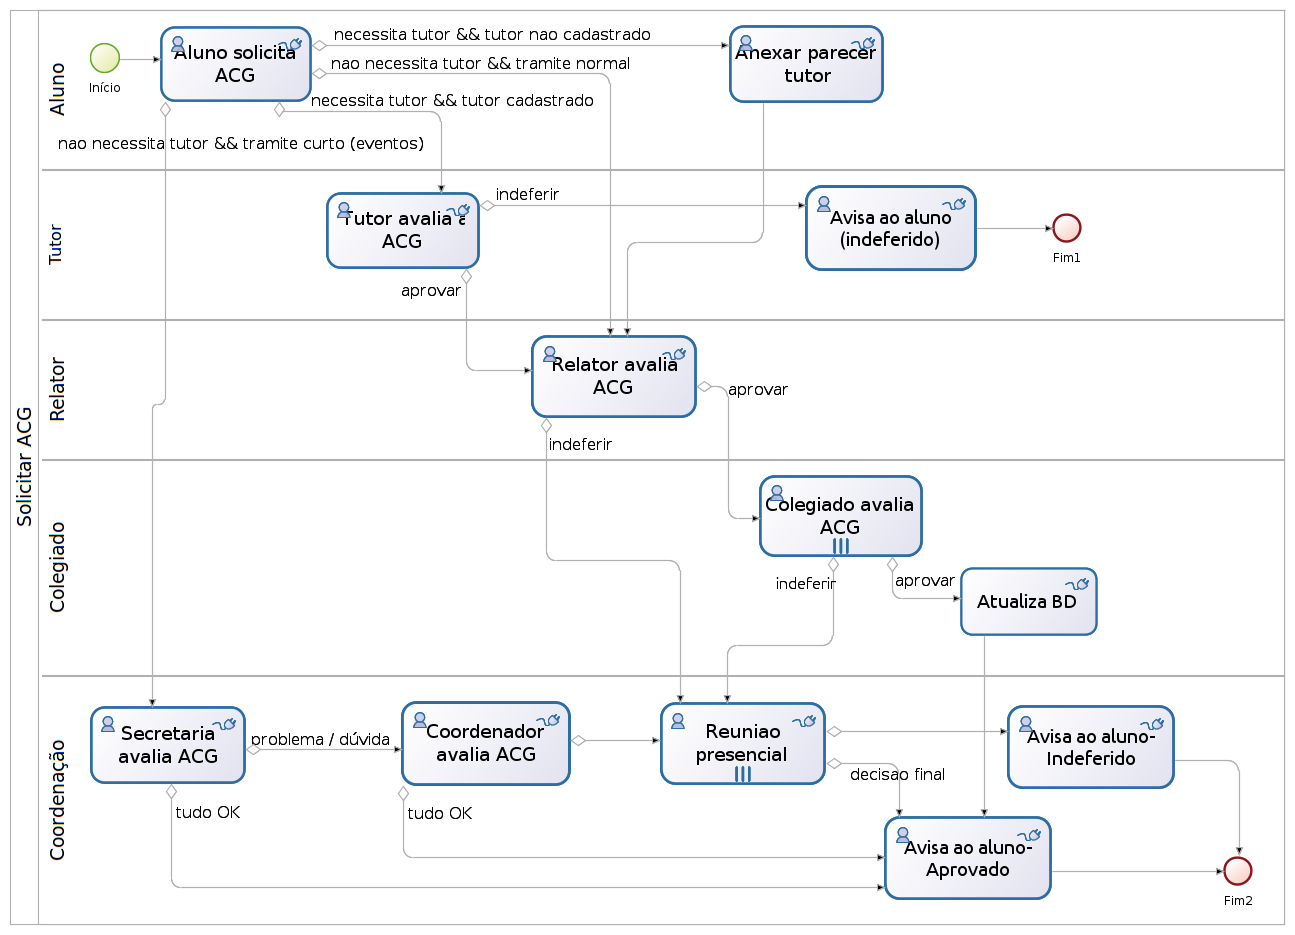
\includegraphics[width=.99\textwidth]{images/processo.png}
\caption{Diagrama da modelagem do processo}
\label{fig:diagrama}
\end{figure}

\subsection{Implementação}

% forms e customizações
% gestão de documentos
% integracao com ldap
% relatorios
% BD
% personalizacao interface

Um dos primeiros passos durante a implementação foi a criação dos formulários a serem visualizados pelos participantes, conforme os papéis que desempenham. No Bonita Studio, a construção de formulários é facilitada, pois existem vários tipos de elementos pré-definidos que como caixa de texto, campo de data ou uma lista, por exemplo. Utilizando dos elementos citados, é possível construir rapidamente um formulário. Porém, no caso prático em questão, foi necessário realizar algumas customizações através de código na linguagem Groovy, para atender alguns requisitos tais como: geração de uma lista com possíveis professores/tutores, auto-preenchimento das informações dos alunos, etc. A figura \ref{fig:form}  mostra um exemplo de formulário visualizado pelo aluno, no momento em que este realiza a solicitação de aproveitamento de ACG.

\begin{figure}[ht]
\centering
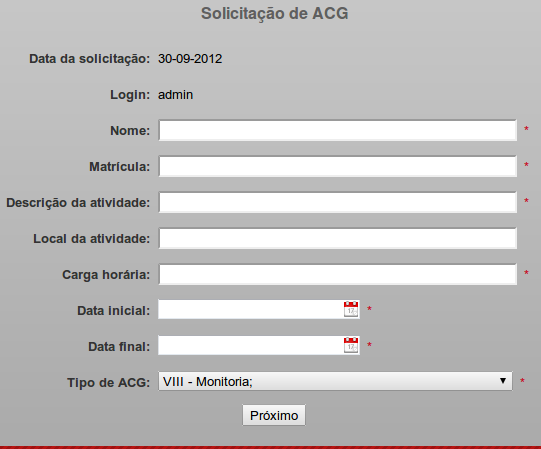
\includegraphics[width=.9\textwidth]{images/formSolicitacao.png}
\caption{Formulário de solicitação de aproveitamento}
\label{fig:form}
\end{figure}

Para que o aluno pudesse enviar os documentos comprobatórios (certificados, atestados, pareceres, etc), utilizou-se um sistema para gestão de conteúdo empresarial, do inglês Enterprise Content Management (ECM), denominado Alfresco \cite{ALFRESCO}. Essa tecnologia foi escolhida por ser suportada via um conector na plataforma BOS, permitindo assim um gerenciamento facilitado dos documentos mesmo após o término dos processos (o que de fato é necessário, pois tais documentos precisam ser arquivados na instituição). Tal como BOS, Alfresco também é um software livre, desenvolvido em Java e com interface Web.

Para a implementação do cadastro e login dos participantes do processo como usuários do sistema, foi utilizada a própria plataforma de execução provida pelo BOS. Como os usuários já se encontravam cadastrados em outros sistemas na instituição, buscou-se uma solução que permitisse utilizar os mesmos nomes e senhas de usuário. Assim, optou-se autenticar usuários através de uma base de dados LDAP, do inglês Lightweight Directory Access Protocol, implementada pelo serviço Linux OpenLDAP. Os demais serviços da subunidade também utilizam essa base de dados, visando centralizar informações e evitar redundância e inconsistência de dados.

Para implementar a autenticação via LDAP, foi criado um novo módulo de login para o BOS, baseado em códigos Java retirados dos fóruns de discussão da ferramenta. Esse módulo substitui o módulo padrão de login, o qual autentica usuários através de um banco de dados interno à plataforma de execução. Paralelamente, foi necessário cadastrar grupos de usuários diretamente no BOS, pois muitas atividades dependiam dessa vinculação de usuários a grupos, e tais grupos não existiam na base LDAP. Os grupos criados foram “tutores”, “relatores”, “colegiado” e “coordenação”, correspondendo às divisões de responsabilidade no processo. Também foi necessário vincular usuários ao grupo “admin”, que é um grupo padrão no BOS para designar usuários com permissões administrativas sobre os processos.

Outro ponto importante na implementação do processo foi a geração de relatórios voltados tanto para alunos como para a coordenação, tais como histórico de solicitações de ACGs e resumo de carga horária homologada e faltante ao currículo do aluno. A ferramenta BOS possui um tipo de conector que utiliza a biblioteca JasperReports para a geração de relatórios associados a um processo \cite{JASPERSOFT}. Tal conector, no entanto, busca os dados do relatório em uma base de dados externa à base do BOS.

A partir da necessidade de relatórios, portanto, foi preciso definir uma base de dados externa para o armazenamento das informações de solicitação/apreciação de atividades. Iniciou-se definindo a estrutura relacional contendo as seguintes tabelas: acg, avaliacao\_colegiado, avaliacao\_relator, avaliacao\_sec\_coord, avaliacao\_tutor e tipo\_acg, conforme mostra a figura \ref{fig:bd}. Em seguida, foi escolhido o SGBD Java H2 pela simplicidade e eficiência. Depois disso, foi necessário incluir conectores do SGBD H2 em tasks do processo, com as respectivas consultas SQL, para que a base de dados de atividades ficasse constantemente atualizada, sendo assim uma fonte segura para os relatórios.

\begin{figure}[ht]
\centering
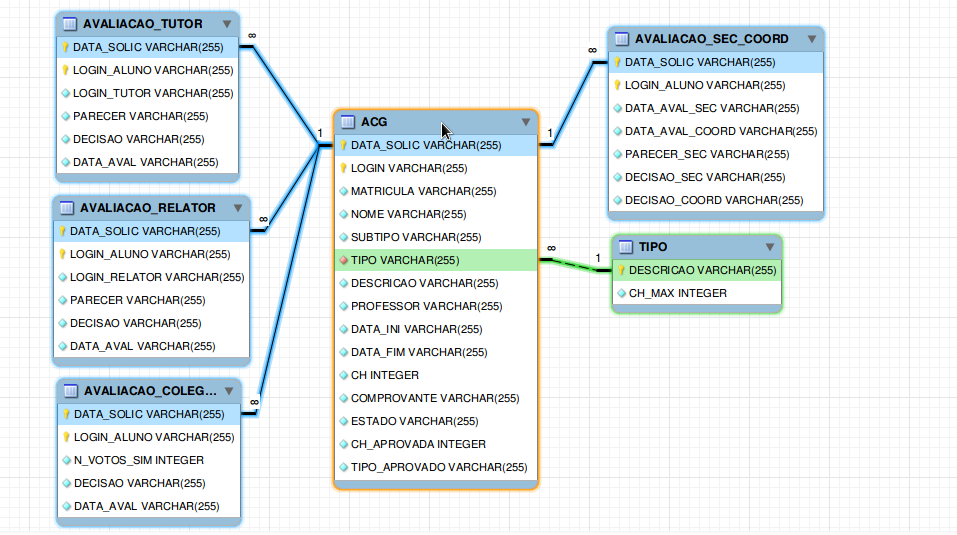
\includegraphics[width=.8\textwidth]{images/bancoLogico.png}
\caption{Modelo lógico relacional da base de dados}
\label{fig:bd}
\end{figure}

Para a implementação dos relatórios, foi necessário construir uma definição XML (contendo as consultas SQL, definições de campos, formatações, etc.)  para cada relatório utilizando a ferramenta gráfica iReport. Mais tarde, essas definições são executadas pela biblioteca JasperReports também provida por Bonita através do conector, contra uma fonte de dados. Para que os usuários tivessem acesso aos relatórios gerados, foram criados mais dois processos chamados “Listar ACGs do usuário” (histórico) e “Resumo ACGs do usuário” (carga-horária). A figura \ref{fig:reports} ilustra esse mecanismo de funcionamento básico de conectores BOS para geração de relatórios com a biblioteca JasperReports.

\begin{figure}[ht]
\centering
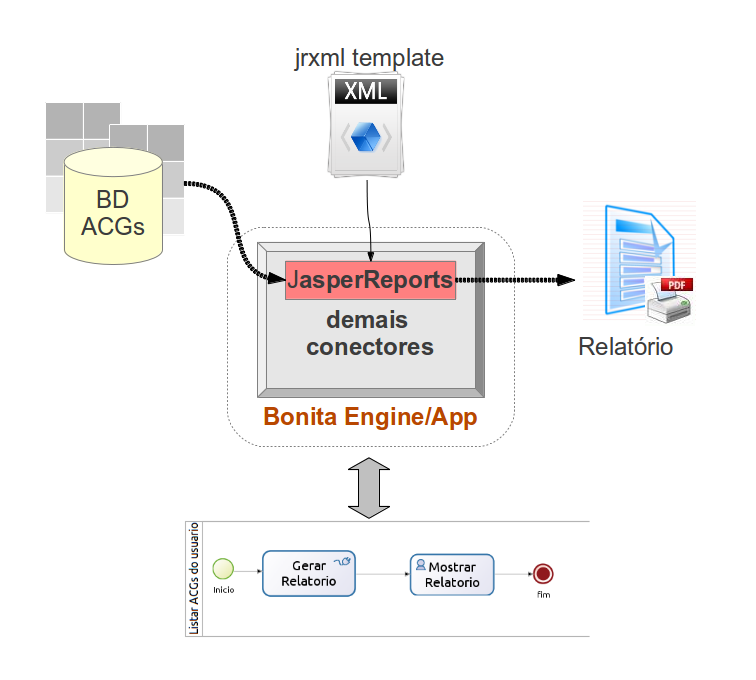
\includegraphics[width=.5\textwidth]{images/conector.png}
\caption{Funcionamento do conector que gera relatórios}
\label{fig:reports}
\end{figure}


A última etapa da implementação foi a personalização da interface do sistema, substituindo imagens e cores padrão do ambiente por elementos que remetem à identidade visual da instituição. Esta customização foi realizada alterando-se arquivos HTML e CSS que definem a interface Web do BOS. Outras personalizações mais profundas também foram necessárias na interface, para remover componentes julgados desnecessários, que acabavam por confundir os usuários. Porém, estas alterações não poderiam ser feitas apenas editando-se imagens e arquivos. Neste caso, foi necessário a alteração do código do próprio BOS, algo que só foi possível pelo fato de a ferramenta ser distribuída como software livre.


Ao longo do desenvolvimento, foi criado um repositório on-line, disponível em http://code.google.com/p/bpm-infufsm/. Nesse repositório, encontram-se todos os artefatos produzidos durante o desenvolvimento do trabalho (lista de requisitos, modelo do processo, versões do código implementado, esquemas de banco de dados, etc.). O repositório também permite que usuários registrem dúvidas, problemas ou sugestões relacionadas ao software.

% Nesta etapa, foi necessário a criação de scripts para início automático dos serviços (Alfresco, Tomcat, BOS, Banco de Dados), que não são fornecidos junto com o software.

\section{Avaliação}

Após a implementação foi iniciada a fase de testes com usuários finais (membros do colegiado e alguns alunos). Os testes realizados ao longo do desenvolvimento indicaram aceitação por parte dos usuários e revelaram oportunidades de melhoria da interface e da modelagem do processo. Após várias revisões, teve início a fase de implantação do processo, permitindo avaliá-lo em relação aos objetivos iniciais.

O processo foi disponibilizado à comunidade do curso, envolvendo cerca de 120 alunos e 25 professores. Logo no primeiro mês, o sistema registrou mais de 100 instâncias (casos abertos) do processo. Em consultas informais aos usuários, notou-se forte aceitação da abordagem utilizada, que evita trâmite de documentos em papel. A experiência com BOS no caso em questão foi apresentada a alunos de uma disciplina sobre modelagem de processos de negócio, suscitando interesse e reconhecimento. Entende-se, portanto, que todos os objetivos foram atingidos.

Mesmo com uma avaliação positiva, a implantação revelou alguns problemas. O principal deles diz respeito a casos que falham, por exemplo devido a problemas de comunicação com o gerenciador de documentos (Alfresco) ou com o banco de dados. Na implementação atual, os casos falhos são simplesmente assinalados aos usuários, sem uma explicação para isso. A identificação do motivo da falha só é possível pela análise de \emph{logs} do BOS, sendo muitas vezes difícil de localizar. É possível alterar a modelagem para incluir caminhos alternativos em caso de falhas, mas isso torna o processo mais complexo e não resolve todos os tipos de problemas (por exemplo, \emph{bugs} no processo). Tudo isso revela a importância de se realizar muitos testes com o processo. Testes automatizados, no entanto, não são suportados pela ferramenta. Independentemente disso, é importante utilizar alguma ferramenta externa para gerenciamento de defeitos e mudanças. No caso em questão, utiliza-se o \emph{issue tracker} disponível no repositório do projeto, em http://code.google.com/p/bpm-infufsm/issues.

De modo geral, a experiência com o BOS foi bastante positiva. Todas as características que levaram à escolha desse BPMS foram comprovadas na prática. Alguns recursos do BOS possuem documentação escassa (por exemplo, integração com LDAP e geração de relatórios) e só puderam ser utilizados com auxílio do fórum de discussão da ferramenta, consumindo tempo significativo de desenvolvimento. Uma necessidade que surgiu durante o trabalho foi a edição colaborativa de um processo, já que a equipe tem mais de um desenvolvedor. Isto é previsto em uma versão comercial do software (Bonita Subscription Pack), mas não no BOS. Mesmo assim, foi possível criar uma estratégia manual de compartilhamento e controle de versão com Subversion, utilizando um cliente e um servidor externos.

Com o sistema em pleno funcionamento, a interface administrativa do BOS, mostrada na figura \ref{fig:interfaceadm}, revelou algumas limitações. Por exemplo, quando se tem uma grande quantidade de casos abertos, torna-se difícil organizá-los ou localizar um caso específico. Em uma versão comercial do software existe a opção de filtragem e busca dos casos mas, novamente, isso não está disponível no BOS. Porém, com a experiência adquirida, estima-se que o problema possa ser resolvido através de relatórios.

\begin{figure}[ht]
\centering
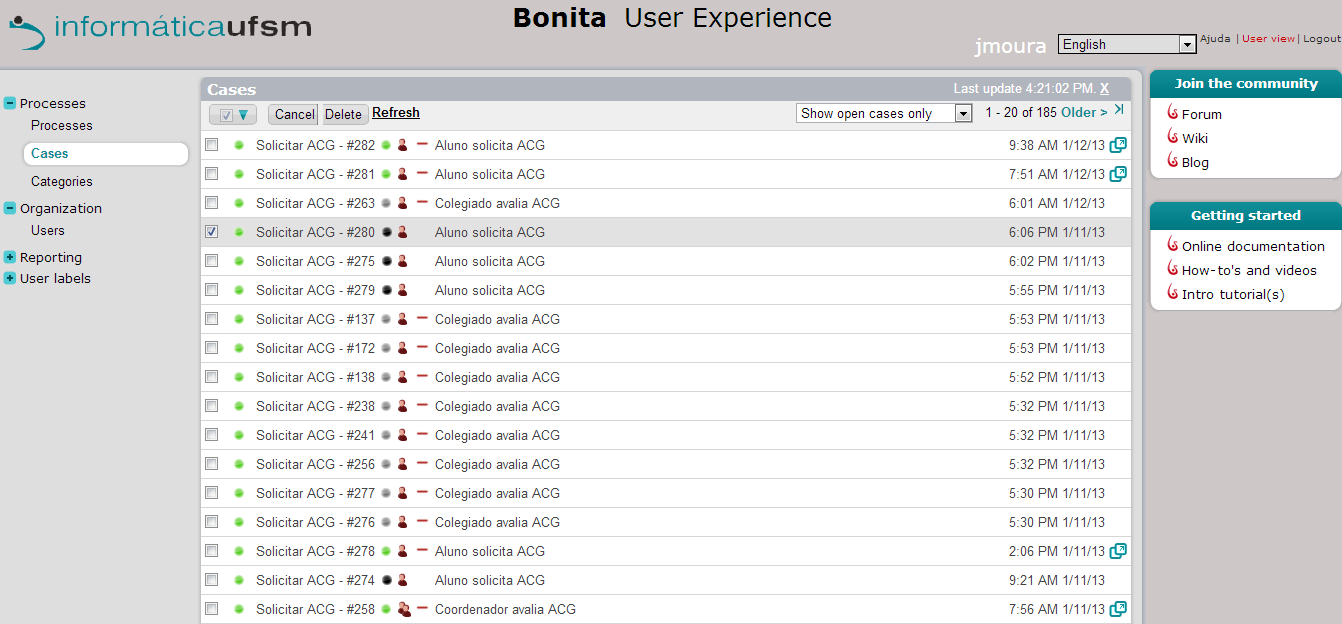
\includegraphics[width=.99\textwidth]{images/interfaceAdministrativa.png}
\caption{Interface Administrativa}
\label{fig:interfaceadm}
\end{figure}

\section{Considerações Finais}

Este trabalho abordou um caso prático de aplicação de conceitos de BPM e ferramentas BPMS, inserido na realidade de cursos de graduação. Como contribuições, o trabalho traz a modelagem e implementação de um sistema baseado em tecnologias de BPM, visando melhorar um processo que é realizado com bastante frequência em uma instituição de ensino superior e, mais especificamente, no âmbito de um curso de Sistemas de Informação. O sistema desenvolvido foi implementado levando em conta o processo de apreciação de ACGs em uma instituição específica, mas a ferramenta permite que ele seja adaptado a outras instituições de ensino superior submetidas à mesma legislação.

Outra contribuição deste trabalho está na exploração da ferramenta Bonita Open Solution, onde pode-se explorar toda a potencialidade da ferramenta, utilizando-se do fato de ser um software livre para modificar o código do programa de acordo com as necessidades. Além de incentivar o interesse de alunos por essa ferramenta, o trabalho mostrou que a ferramenta é eficiente para a melhoria de um processo real.

Como trabalhos futuros, pretende-se dar continuidade na exploração de BPM e suas contribuições para melhoria de processos internos ao curso. Além disso, pretende-se manter a contínua documentação dos passos realizados na transformação dos processos, incluindo detalhes de projeto, implementação e, também, de testes com usuários finais. Isso irá reforçar um exemplo real de aplicação de BPM, disponível em repositório on-line, para alunos de Sistemas de Informação e áreas afins.


\bibliographystyle{sbc}
\bibliography{sbc-template}

\end{document}
